%!TEX root = ../vernier.tex
\section{Visualizing Evolution} \label{sec:evolution}
So far we are able to reason about the similarity of entities, their hierarchical relationships, their current metric values for any given collected revision, and the metric value change from revision $t_{i}$ to $t_{i+1}$. What we yet cannot do is to intuitively display the evolution of a set of entities throughout large time intervals. With this in mind, we've implemented two visualization techniques.

The first is the Streamgraph, inspired on the design present on the SolidTA tool \cite{ref:solid} illustrated on figure \ref{fig:flow_solid}. It subdivides the screen space vertically into $R$ sections, where $R$ is the number of revisions being analyzed. Then, for an arbitrary number of selected classes, it draws a lines where the height at any given time subdivision represents the  value of a chosen metric at that moment. This information can be emphasized by color coding (with one the colormaps introduced on section \ref{sec:colormap}) the line section with the same metric attribute, as exemplified on figures \ref{fig:stream_10_loc} and \ref{fig:stream_10_loc_div} for 10 entities of the ExoPlayer project and the lines of code metric between the December 2014 and February 2016.

\begin{figure}[H]
	\centering
	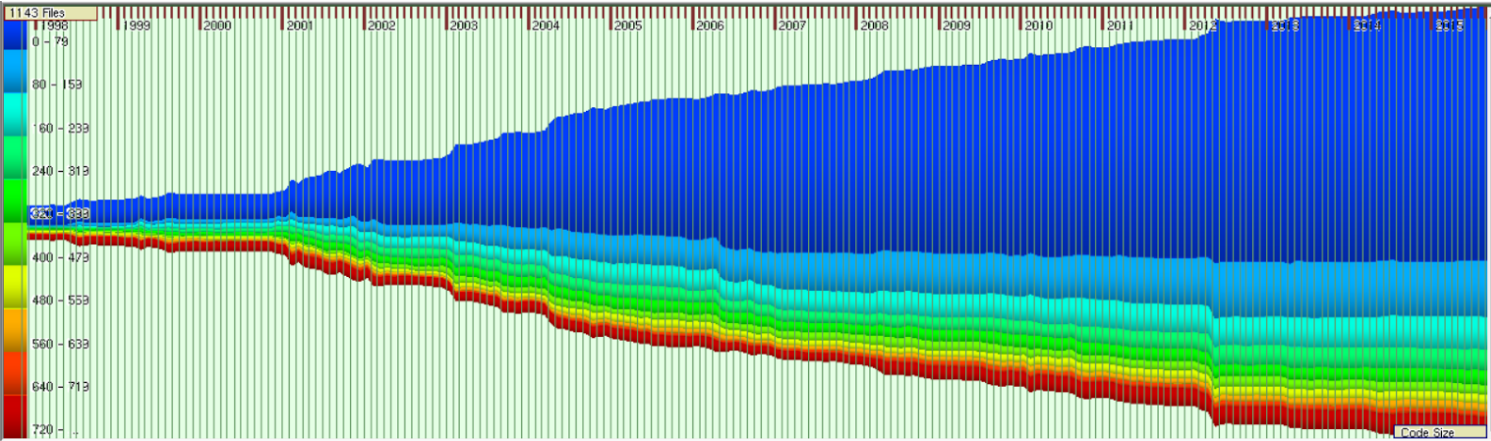
\includegraphics[width=1.0\textwidth]{figures/flow_graph.png}
	\caption{Evolution of the file count on the GIMP project color coded by file size using SolidTA}
	\label{fig:flow_solid}
\end{figure}


\begin{figure}[H]
	\centering
	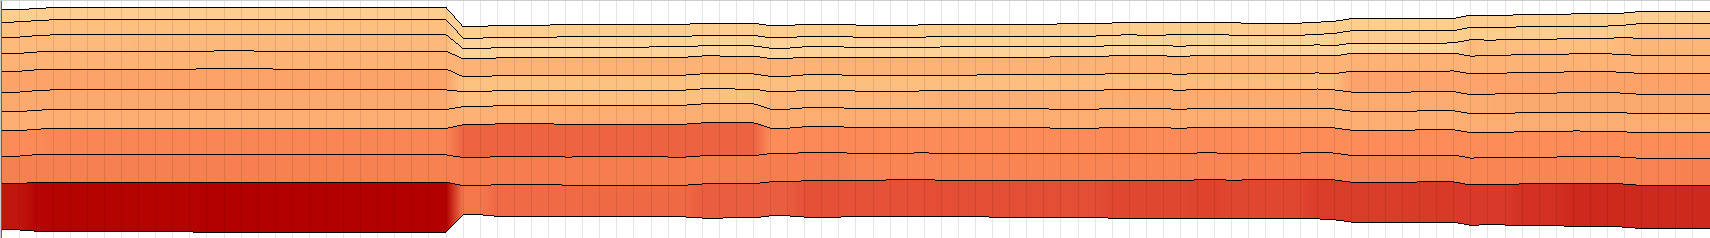
\includegraphics[width=1.0\textwidth,height=4.0cm]{figures/stream_10_loc.png}
	\caption{Evolution of the LOC metric for 10 classes using the sequential colormap}
	\label{fig:stream_10_loc}
\end{figure}

\begin{figure}[H]
	\centering
	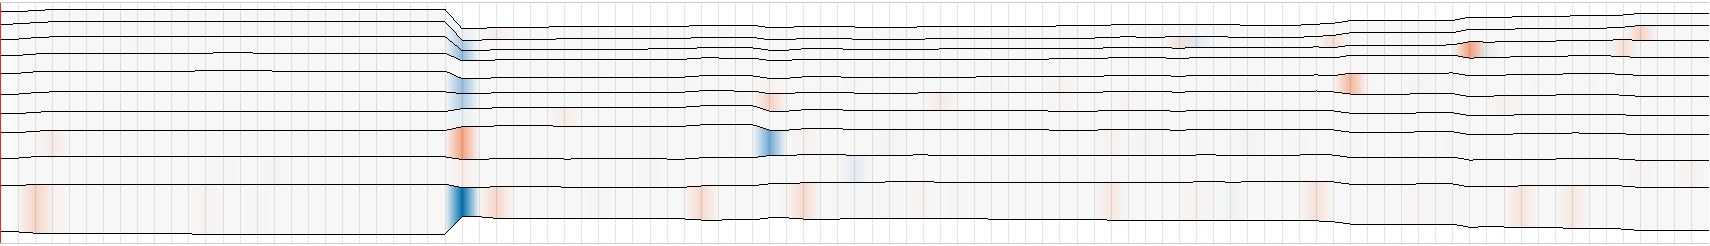
\includegraphics[width=1.0\textwidth,height=4.0cm]{figures/stream_10_loc_div.png}
	\caption{Evolution of the LOC metric for 10 classes using the divergent colormap}
	\label{fig:stream_10_loc_div}
\end{figure}

One characteristic of the Streamgraph is that it can naturally represent the global evolution of an attribute through time. Figure \ref{fig:stream_all_loc} shows the evolution of the LOC metric on ExoPlayer for the 15 earlier mentioned months. The biggest insight that we can extract from this visualization is not about ExoPlayer, but about our own technique.

Software projects grow and, using \textit{git checkout} commands and the CLOC tool %TODO add ref
, we discovered that in the analyzed period of time the project has evolved from 18.4KLOC (thousand of lines of Java code) to 42.2KLOC, almost doubling the number of classes from 169 in December 2014 to 332 in February 2016. Yet, due to the filtering process (see section \ref{sec:filtering}) that is imposed given the limitations of state of the art projection techniques, we can't see this change, supposedly because we were only able to analyze 117 of the total number of classes. Additionally, one can argue (and later, on figure \ref{fig:spectro_exo}, confirm) that our classes are in a very stable state (fact that might relate to their time of creation) and that the time classes evolve the most is right after their creation.

\begin{figure}[H]
  \centering
  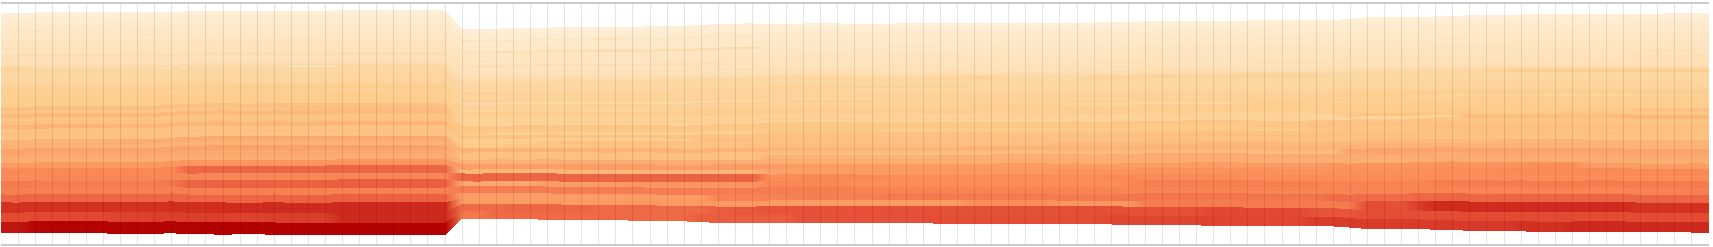
\includegraphics[width=1.0\textwidth,height=4.0cm]{figures/stream_all_loc.png}
  \caption{Filtered evolution of the LOC metric on ExoPlayer from Deceber 2014 to February 2016}
  \label{fig:stream_all_loc}
\end{figure}

The impression given by our visualization is that the size of the project hasn't increased significantly during the studied period, but we know that this is not true. In fact, an increase of 129\% in the number of lines of code has taken place during this time.

This artifact is not a one-off occurrence, the same can be seen on projects such as RxJava (figure \ref{fig:stream_rxjava}), Google Closure (figure \ref{fig:stream_closure}), and Eclipse Vert.x (figure \ref{fig:stream_closure}).

\begin{figure}[H]
  \centering
  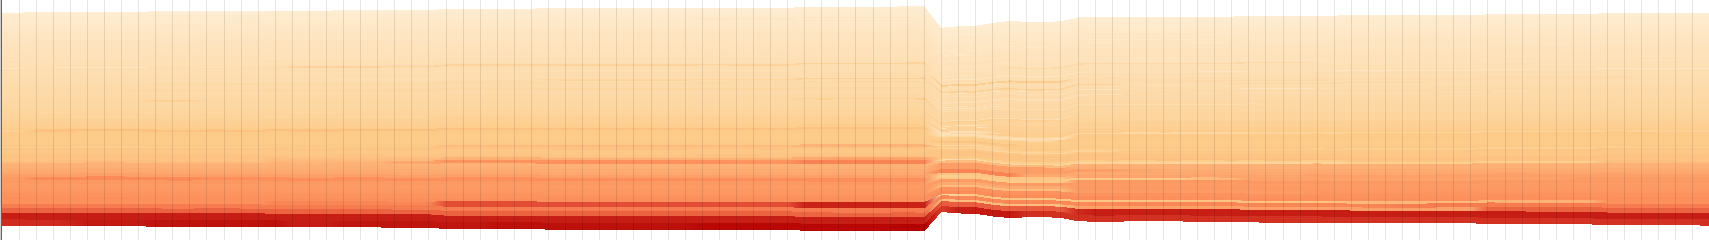
\includegraphics[width=1.0\textwidth,height=4.0cm]{figures/stream_rxjava.png}
  \caption{Filtered evolution of the LOC metric on the RxJava project from December 2013 to February 2016}
  \label{fig:stream_rxjava}
\end{figure}

\begin{figure}[H]
  \centering
  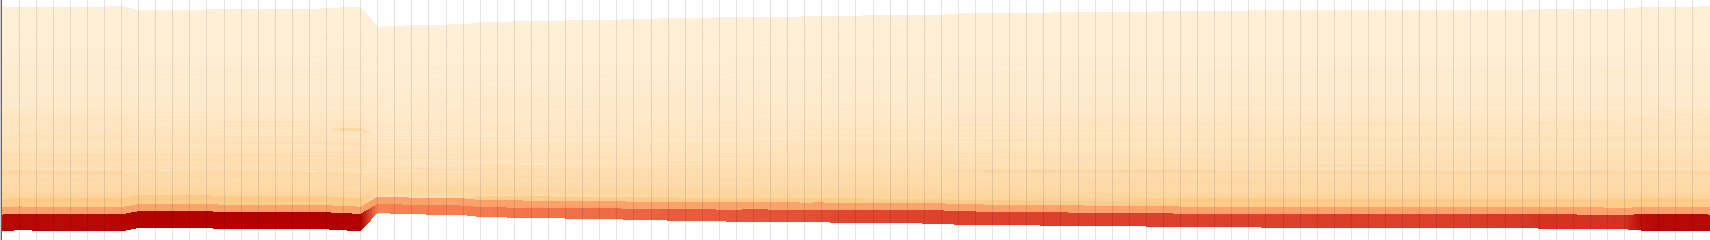
\includegraphics[width=1.0\textwidth,height=4.0cm]{figures/stream_closure.png}
  \caption{Filtered evolution of the LOC metric on the Google Closure project from August 2011 to February 2016}
  \label{fig:stream_closure}
\end{figure}

\begin{figure}[H]
  \centering
  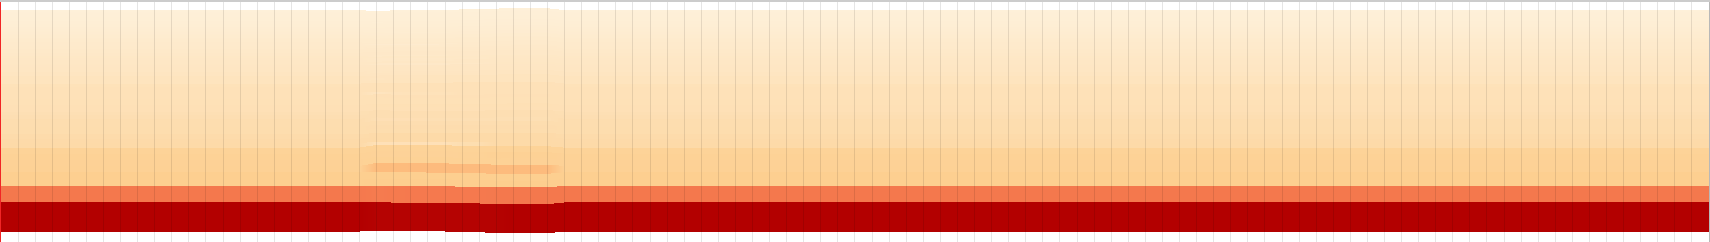
\includegraphics[width=1.0\textwidth,height=4.0cm]{figures/stream_vertx.png}
  \caption{Filtered evolution of the LOC metric on the Eclipse Vert.x project from January 2014 to February 2016}
  \label{fig:stream_vertx}
\end{figure}

This artifact is a result of the filtering process, but not all datasets need filtering. Imagine a time dataset that consist of atmospheric, fluvial, pluvial, fauna, flora, as well as other terrain related attributes. In this case, there wouldn't be a problem, as there is no creation or deletion of terrains.

The other evolution visualization tool we implemented is the Spectrograph. In contrast to the Streamgraph, it uses a fixed line height and relies solely on color to communicate metric value at each instant. The Spectrograph excels at presenting the distribution of the data and element-wise evolution. Additionally, similar to the Treemap, it is uses all "real state" available for display of data.

Figure \ref{fig:spectro_exo} is different portrayal of the same data on figure \ref{fig:stream_all_loc}. It confirms our suspicions about the stability of the data points.

\begin{figure}[H]
  \centering
  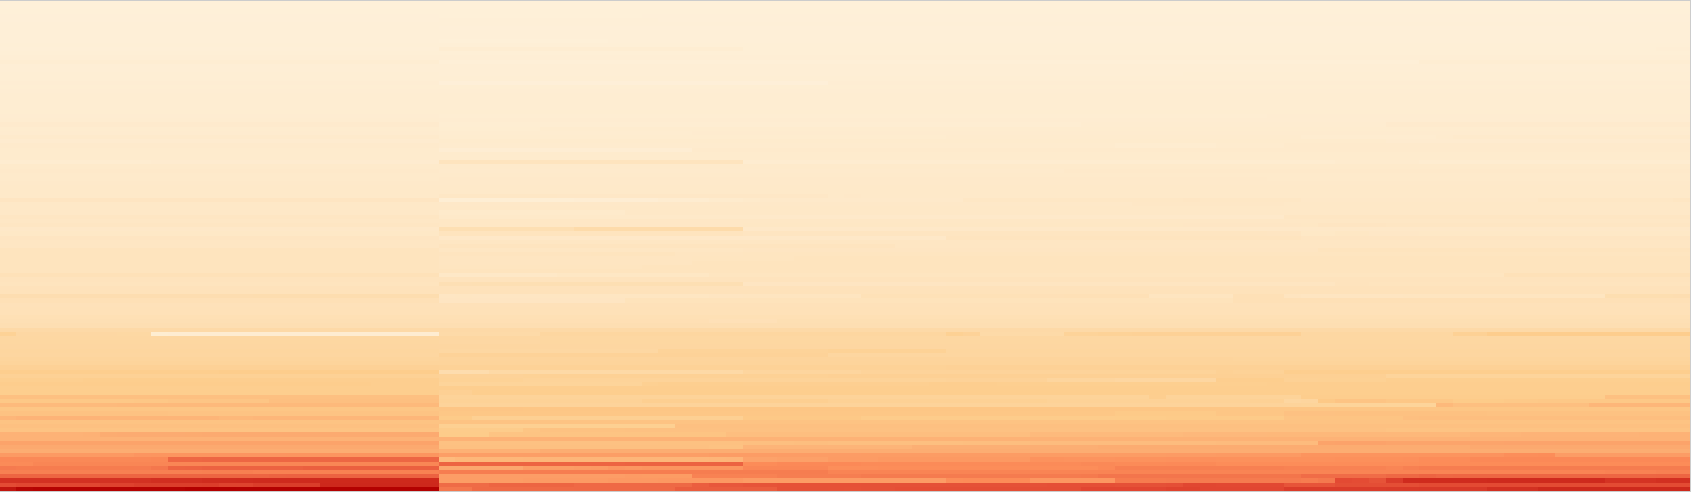
\includegraphics[width=1.0\textwidth]{figures/spectro_exo.png}
  \caption{Filtered evolution of the LOC metric on ExoPlayer from Deceber 2014 to February 2016}
  \label{fig:spectro_exo}
\end{figure}

Similar to the Streamgraph, the Spectrograph can show the evolution of any metric for a set of entities. In figures \ref{fig:spectro_lack_exo} and \ref{fig:spectro_lack_rxjava}, we compare the distribution of the Percent Lack Of Cohesion metric distributions between the ExoPlayer and RxJava projects. Cohesion is an important concept in OOP \cite{chidamber1994}, as it indicates whether a class represents a single abstraction or multiple abstractions. Cohesiveness of methods within a class is desirable, since it promotes encapsulation. Lack of cohesion suggests that classes should probably be split into two or more sub-classes, decreasing complexity and reducing the likelihood of errors during the development process. Therefore, through this somewhat inelegant metric name, we get the understanding that lower metric values represent a better situation. What means that the RxJava project (or at least it's filtered classes) has a better, least prone to errors, design than ExoPlayer.

\begin{figure}[H]
  \centering
  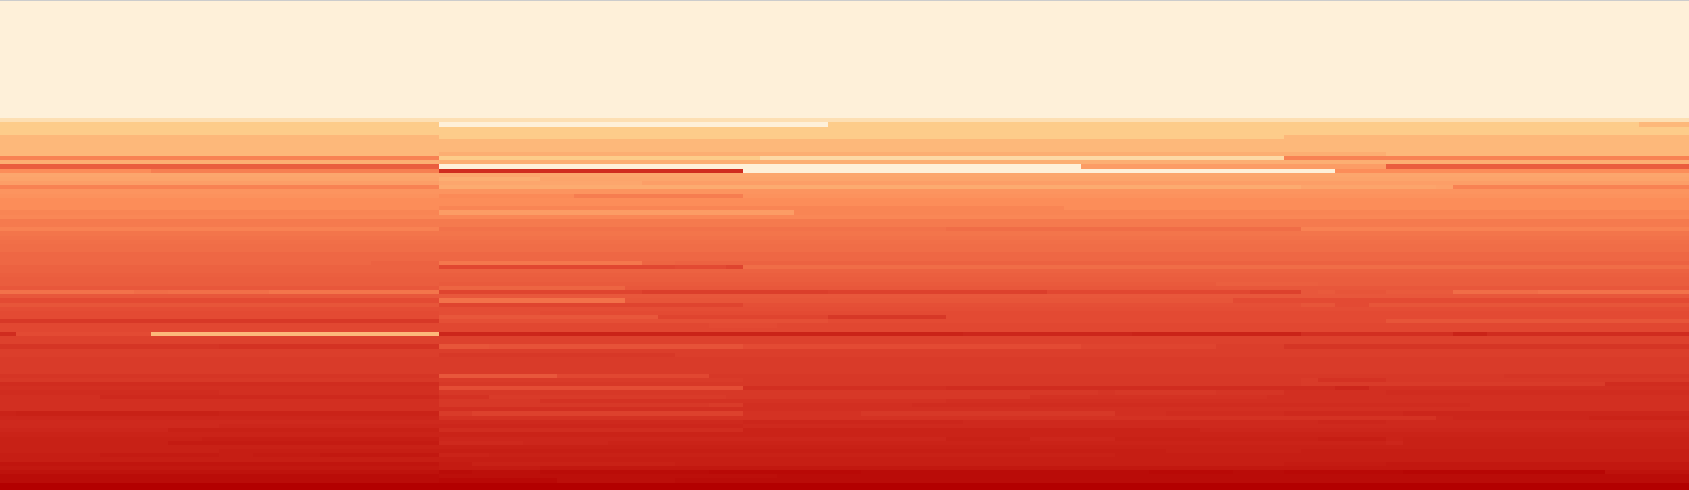
\includegraphics[width=1.0\textwidth]{figures/spectro_lack_exo.png}
  \caption{Filtered evolution of the PercentLackOfCohesion metric on the ExoPlayer project.}
  \label{fig:spectro_lack_exo}
\end{figure}

\begin{figure}[H]
  \centering
  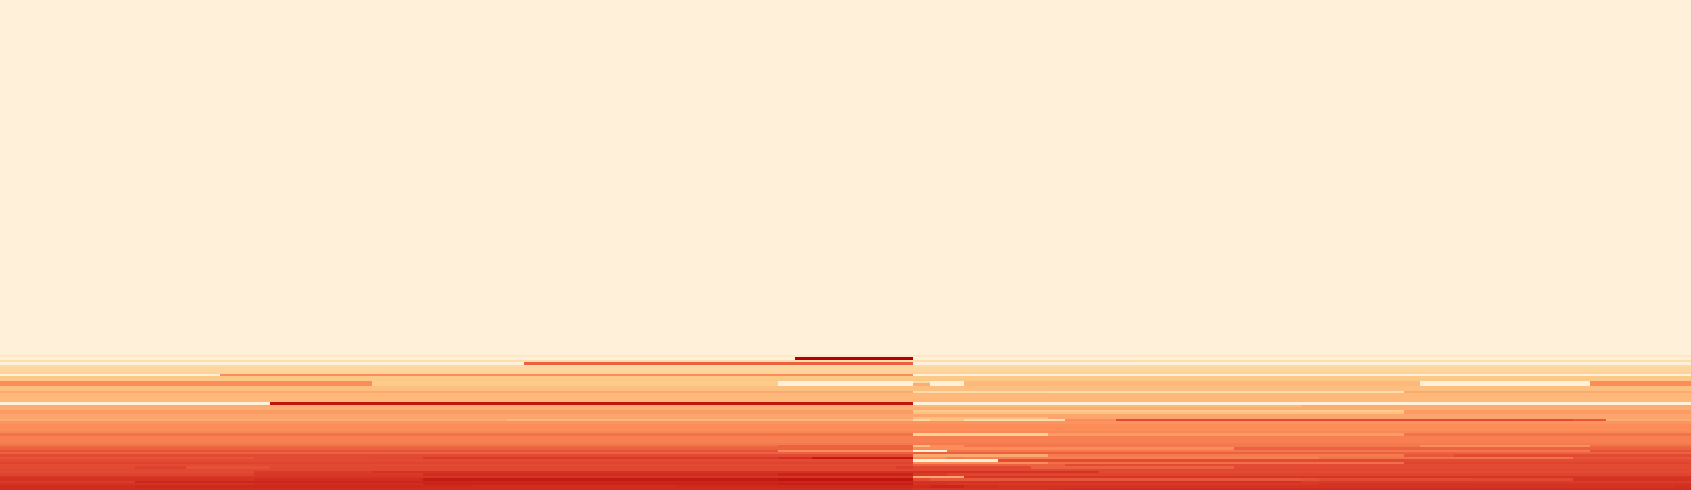
\includegraphics[width=1.0\textwidth]{figures/spectro_lack_rxjava.png}
  \caption{Filtered evolution of the PercentLackOfCohesion metric on the RxJava project.}
  \label{fig:spectro_lack_rxjava}
\end{figure}
